\documentclass[]{article}
\usepackage[margin=1in]{geometry}
\usepackage{nopageno}
\usepackage{graphicx}
\usepackage{amsmath}
\usepackage[labelfont=bf]{caption}
\usepackage[utf8]{inputenc}
\usepackage[english]{babel}
\usepackage{amsthm}
\graphicspath{ {figures/} }

\newtheorem{theorem}{Theorem}
\newtheorem{claim}[theorem]{Claim}
\newtheorem{proposition}[theorem]{Proposition}
\newtheorem{lemma}[theorem]{Lemma}
\newtheorem{corollary}[theorem]{Corollary}
\newtheorem{conjecture}[theorem]{Conjecture}
\newtheorem*{observation}{Observation}
\newtheorem*{example}{Example}
\newtheorem*{remark}{Remark}

%opening
\title{In-Depth Statistical Analysis of Ritwik Distribution}
\author{\{Ritwik, Ritwik, Ritwik\} Gupta, Das, Rajendra\footnote{Authors are listed in the order of narcissism towards their first names}
	\\
	\{ritwikg1, rsdas, ritwikr\} @ andrew.cmu.edu
	\\
	\\
	The Council of Ritwiks @ Carnegie Mellon}
\date{}

\begin{document}

\maketitle

\begin{abstract}
The distribution of Ritwiks across the world is a question pursued by countless researchers across a variety of fields. A yet unanswered question\footnote{https://scholar.google.com/scholar?hl=en\&as\_sdt=0\%2C39\&q=distribution+of+ritwiks\&btnG=}, we seek to once and for all put this question to rest. We also provide auxiliary discussion and proofs demonstrating various statistical properties of the Ritwik population.
\end{abstract}

\section{Distribution of Ritwiks}
Comprehensive, boots on the ground research was done to effectively determine the distribution of Ritwiks across the world. Using Facebook\footnote{https://facebook.com}, we were able to ascertain the location of and establish contact with Ritwiks everywhere (see Figure \ref{fig:ritwikgeographicaldistro}).
\begin{figure}[h]
	\centering
	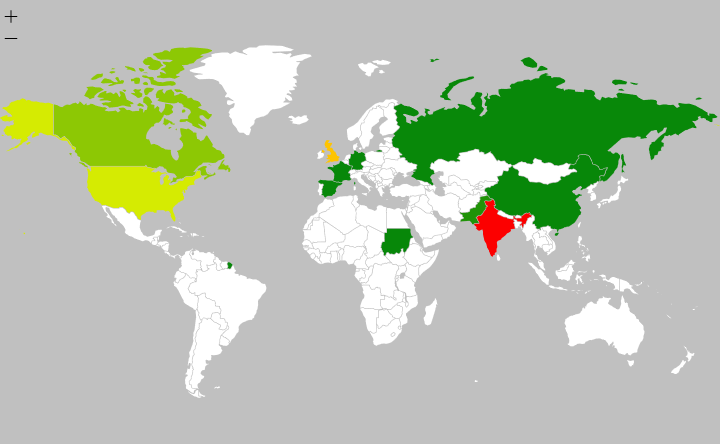
\includegraphics[width=3in]{figures/RitwikGeographicalDistro}
	\caption{Geographical density of Ritwiks, green being low and red being high.The white areas denote the authors were lazy to make a heat map covering the globe.}
	\label{fig:ritwikgeographicaldistro}
\end{figure}
We collected a large sample size ($N = 12$) and used Hamiltonian Monte Carlo methods to simulate certain parameters that are backed by Bayesian goodness, undeniably proving that our method is rock solid. We cast a net out to collect the samples , the deep kind of net therefore guaranteeing the best sample. All data was analyzed with cutting edge tools \cite{Zaharia:2012:RDD:2228298.2228301, PyMC3}. The following math not only looks cool, but makes reviewers think that we did real work because math makes it look that way.
\begin{subequations}
\begin{align}
Count_i \sim Poi(\lambda),\\
\lambda \sim DiscreteUniform(0, 7e9),\\
\int_{\lambda}\pi(q)f(q)\sum{\frac{Var_\pi[f]}{ESS}}
\end{align}
\end{subequations}
\vspace{1in}

\subsection{Estimating the Density of ``Ritwik" Using Novel Methods}
Ritwik is a low frequency name, a statement which has been shown to be true using time-tested methods of Expected Author Intuition Level (EAIL). Li et. al. \cite{Baby} state that low frequency names are related to each other using Zipf's Law which is stated as follows:

\vspace{2mm}
Let $X = \{x_1, x_2, x_3, x_4, x_5, x_6, x_7, x_8, x_9, x_{10}, x_{11}, ... , x_N\}$, $N$ = some large number and $X$ is the vector of names present in the world. Let $Y = \{y_1, y_2, y_3, ... y_N\}$ be the ranking of each $x_i$. Therefore, Zipf's Law states that:

\begin{equation}
Y \propto \frac{1}{Count(X)} + \xi
\end{equation}


Here $\xi$ is a constant which has been included to make us insecure authors feel good about ourselves. Its been set to zero for all purposes of using the equation. \\
We completely ignore this rule though and use deep learning since representation learning solves all problems. Assume a low density uniform prior on the density of Ritwik over geographical locations (which are sorted alphabetically and mapped to whole numbers). When you imagine it in your head, it sure does look like a line, right? Therefore, we use linear activations in our neural network model, leading to a massive gain in performance to competing Ritwik density estimators (see Table \ref{table:affineadversarial} below).

\begin{table}[h]
\centering
\begin{tabular}{|c|c|c|c|}
	\hline
	\textbf{Method} & \textbf{MAP} & \textbf{MRP} & \textbf{GDP} \\
	\hline
	SVM & 0.05 & 0.02 & 9.65 \\
	\hline
	SVM + BBN & 0.45 & 0.21 & 3.21 \\
	\hline
	RBM & 0.68 & 0.44 & 2.96 \\
	\hline
	Linear NN (ours) & \textbf{1.00} & \textbf{0.99} & \textbf{0.01}\\
	\hline
\end{tabular}
\caption{Performance of Ritwik density methods.To generate this table we used rigorous foolproof experimentation techniques like YOLO(You Only Lie Once).}
\label{table:densitycomp}
\end{table}

An example of an architecture we did \textbf{not} use is included below as reference, carefully created in MS Paint for the highest quality rendering and production value.

\begin{figure}[h]
	\centering
	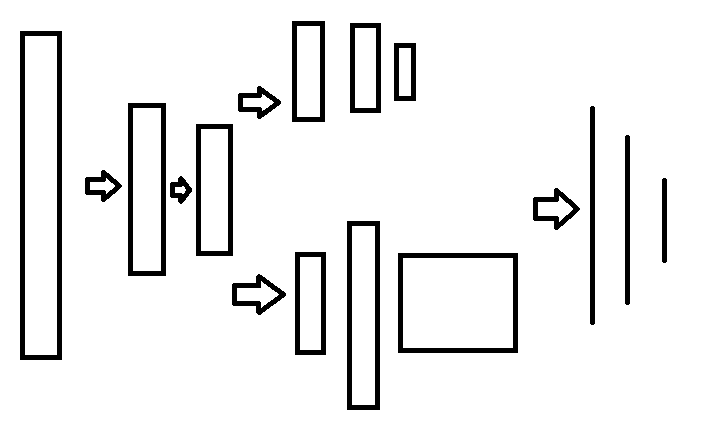
\includegraphics[width=4in]{figures/Neuralnet}
	\caption{An architecture that seems like it would give results, that we summarily ignored.}
	\label{fig:neuralnet}
\end{figure}

To make our results reproducible, we have stuck to well-backed academic practices of releasing all of our code on private GitHub repositories only accessible via an email to one of our auxiliary email addresses that we check once in a blue moon, or after we publish everything of use from the dataset.

\section{Popularity of ``Ritwik" Over Time}
Though Ritwiks themselves are insanely popular\footnote{Refer to our peers.}, the name Ritwik itself has not seen widespread gain in usage throughout history. Using historical databases, we were able to reconstruct the usage of the name and use popular methods such as randomly drawing a line that looks about right to estimate the future usage of the name as well (see \ref{fig:usageofritwik}).
\begin{figure}[h]
	\centering
	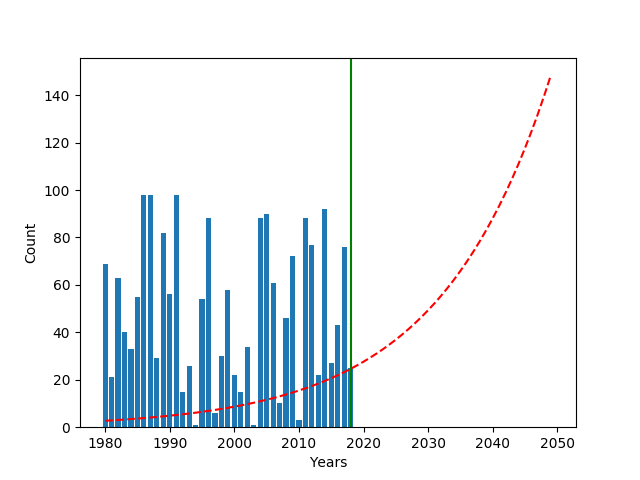
\includegraphics[width=4in]{figures/UsageOfRitwik}
	\caption{The occurrence of the name Ritwik over time. Green line represents the year this paper was published.}
	\label{fig:usageofritwik}
\end{figure}
As evident, the name Ritwik is predicted to skyrocket as this paper is made public. Eventually, all people will be named Ritwik, and the universe will be at peace.

\section{On the Immortality of Ritwiks}
\label{sec:Immortality}
Based on the vast quantity of Ritwiks we have met, none of them have been dead or deceased. As such, we are led to believe that all Ritwiks are immortal until the eventual heat death of the universe \cite{HeatDeath}.
\begin{lemma}
\label{lemma:death}
	Given any Ritwik, the average lifespan of the individual will be $\infty$.
\end{lemma}
\begin{figure}[h]
	\centering
	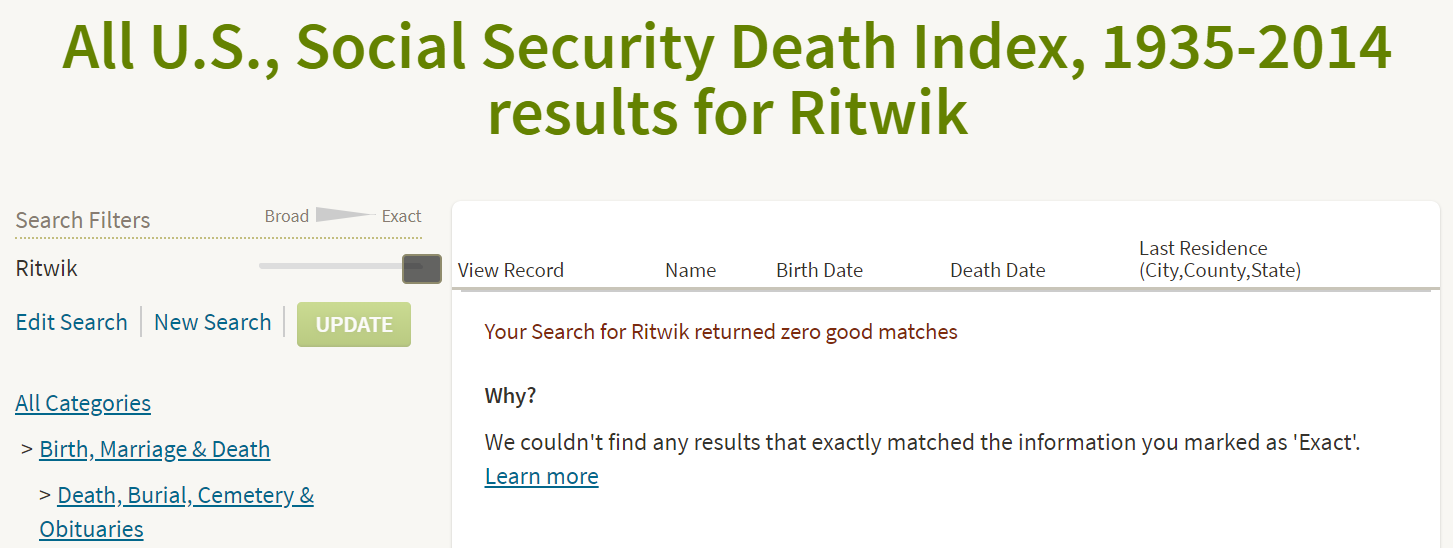
\includegraphics[width=5in]{figures/RitwikLackOfDeath}
	\caption{Search of the U.S. Social Security Death Index for ``Ritwik".}
	\label{fig:ritwiklackofdeath}
\end{figure}
\begin{proof}
Let us assume that all Ritwiks die, for the sake of contradiction. Therefore, a record of death must exist within the United States Social Security Death Index\footnote{http://search.ancestry.com/search/db.aspx?dbid=3693}. However, we can see in Figure \ref{fig:ritwiklackofdeath}, no records of deceased Ritwiks exist. Therefore, Lemma \ref{lemma:death} must hold.
\end{proof}

\section{Adversarial Ritwiks}
With the recent successes in people being able to finally spell our name properly, adversarial attacks against our nomenclature have become prevalent. Simple affine transformations often result in massive confusion amongst peers and colleagues. An example of these transformations can be seen in Table \ref{table:affineadversarial} below.
\begin{table}[h]
\centering
\begin{tabular}{|c|}
	\hline 
	\textbf{Transformation}\\ 
	\hline 
	Rit\textbf{v}ik\\ 
	\hline 
	Ritwi\textbf{c}k\\
	\hline
	\textbf{Rick}\\
	\hline
	\textbf{H}rit\textbf{h}ik\\
	\hline
	\textbf{\textit{``How about I call you Rob?"}}\\
	\hline
\end{tabular}
\caption{Example of affine transformations on the name ``Ritwik"}
\label{table:affineadversarial}
\end{table}
Many defenses exist against adversarial attacks against the name ``Ritwik". Papernot et. al. \cite{Papernot} suggests that distilling these toxic people out of your life demonstrates a sizable increase in the quality of life. However, many attacks have been shown directly bypassing distillation, which means that you're stuck with hearing various people call you different names for the rest of your life, which as shown in Section \ref{sec:Immortality}, is forever.

\section{Conclusion}
We have demonstrated absolutely nothing of use, but are still proud of our contribution to the world. If you are a Ritwik and are currently not a member of the Council, please email us at once to rectify this grave mistake. If you are not named Ritwik this might be a good time to consider a name change. 

\bibliographystyle{unsrt}
\bibliography{references}

\end{document}
